\documentclass{article}
\usepackage{graphicx}
\usepackage{amsmath}
\usepackage{amssymb}
\usepackage{bm}
\usepackage{wrapfig}
\usepackage{float}
\usepackage[a4paper, marginparwidth=0pt]{geometry}
\usepackage{parskip}
\usepackage{lmodern}
\usepackage{pdfpages}
\usepackage[hidelinks,
            unicode,
            pdftitle={Sequence labeling with deep neural networks for natural language processing},
            pdfauthor={Andreas Holck Høeg-Petersen, Frederik Haagensen \& Mathias Bastholm}]{hyperref}
\usepackage{minted}
\usepackage{booktabs}
\usepackage{multirow}
\usepackage[
    backend=biber,
    style=authoryear-icomp,
    eprint=false
]{biblatex}
\usepackage{xstring}
\addbibresource{src/bibliography.bib}

% Better inline directory listings
\usepackage{xcolor}
\definecolor{light-gray}{gray}{0.95}
\newcommand{\code}[1]{\colorbox{light-gray}{\texttt{#1}}}

\graphicspath{{./img/}}

\DeclareMathOperator*{\argmax}{arg\,max}

\title{Sequence labeling with deep neural networks for natural language
processing}
\author{Andreas Holck Høeg-Petersen \and Frederik Haagensen \and Mathias
Bastholm}
\date{2019--05--15}

\begin{document}

\pagenumbering{roman}
% \includepdf{frontpage.pdf}
\begin{titlepage}

\newcommand{\HRule}{\rule{\linewidth}{0.5mm}} % Defines a new command for the horizontal lines, change thickness here

\center % Center everything on the page

%-------------------------------
%	HEADING SECTIONS
%-------------------------------

\textsc{\LARGE IT University of Copenhagen}\\[1.5cm] % Name of your university/college
\textsc{\Large Bachelor Project}\\[0.5cm] % Major heading such as course name
\textsc{\large BIBAPRO1PE}\\[0.5cm] % Minor heading such as course title

%-------------------------------
%	TITLE SECTION
%-------------------------------

\HRule \\[0.4cm]
{ \huge \bfseries Sequence labeling with deep neural networks for natural language processing}\\[0.4cm] % Title of your document
\HRule \\[1.5cm]

%-------------------------------
%	AUTHOR SECTION
%-------------------------------

\begin{minipage}{0.4\textwidth}
\begin{flushleft} \large
\emph{Authors:}\\
%John \textsc{Smith} % Your name
Andreas H. \textsc{Høeg-Petersen} <anhh@itu.dk> \\
Frederik \textsc{Haagensen} <haag@itu.dk> \\
Mathias \textsc{Bastholm} <mbas@itu.dk>
\end{flushleft}
\end{minipage}
~
\begin{minipage}{0.4\textwidth}
\begin{flushright} \large
\emph{Supervisor:} \\
%Dr. James \textsc{Smith} % Supervisor's Name
Leon \textsc{Derczynski} <leod@itu.dk>
\end{flushright}
\end{minipage}\\[4cm]

% If you don't want a supervisor, uncomment the two lines below and remove the section above
%\Large \emph{Author:}\\
%John \textsc{Smith}\\[3cm] % Your name

%-------------------------------
%	DATE SECTION
%-------------------------------

%{\large 23. maj 2017}\\[1cm] % Date, change the \today to a set date if you want to be precise
{\large 2019--05--15}\\[1cm] % Date, change the \today to a set date if you want to be precise

%-------------------------------
%	LOGO SECTION
%-------------------------------


\includegraphics[width=10cm]{logo}\\[1cm] % Include a department/university logo - this will require the graphicx package

%----------------------------------------------------------------------------------------

\vfill % Fill the rest of the page with whitespace

\end{titlepage}

% \maketitle
\pagebreak
\tableofcontents
\pagebreak


\pagenumbering{arabic}

\begin{abstract}

Sequence labeling is a fundamental task in natural language processing and there
exists several renowned machine learning models that achieve state-of-the-art
results on such tasks. In this thesis, we examine two such models, a
bidirectional LSTM model with and without a Conditional Random Field, and see
how the perform on a number of different languages. We limit the scope to
include the part-of-speech tagging task and the named entity recognition task,
and we implement and review the models in three different machine learning
frameworks, DyNet, PyTorch and TensorFlow. We define several configurations and
perform a total of 3780 experiments, and we give an introductory description of
the theoretical and empirical background of the models used and the parameters
used in our configurations. Our results show, that it is possible to achieve
strong performance by applying CRF to the standard bidirectional LSTM, but also
that this advantage diminishes if 2 bidirectional LSTMs are combined. We also
observe, that batch sizes have an impact on both the accuracies of the models
and the time it takes for the models to converge. Furthermore, we find that the
pre-trained Polyglot word embeddings are ill-suited for certain data sources for
Japanese part-of-speech data. Finally, we give suggestions for improvements
based on our findings, and we give individual reviews of the frameworks used for
implementations.

\end{abstract}

\section{Introduction}

\subsection{Project background}


The project was conducted as a bachelor thesis as part of the Software
Development programme at the IT University of Copenhagen. The project period ran
from February 2nd to May 15th 2019. Originally, the attached supervisor was
Zeljko Agic, who was involved in deciding the scope and the main problems of the
project. Early in the process, however, he was substituted with Leon Derczynski
of the Department of Computer Science at the IT University of Copenhagen, who
supervised the project group until submission and examination.

The code, report and results of the project are available at the projects GitHub
repository at \url{https://github.com/anhh-haag-mbas/sequence-labeling}.


\subsection{Project description}

Some of the most fundamental machine learning applications in natural language
processing (NLP) are performing sequence labelling on sentences by processing
one word at a time and attribute it some label. A lot of ingenuity has been put
into designing machine learning models that specializes in tasks like these and
most popular machine learning framework supports these models.

In this project, we aim to examine and compare the performance of two of the
most successful such models, namely a bidirectional Long-Short Term Memory
network (LSTM) and a bidirectional LSTM with an added Conditional Random Field
(CRF) layer. We want to test how they manage part-of-speech tagging (POS) and
named entity recognition (NER), two traditional sequence labelling tasks, and
how different configurations of the training time and batch size affect this. We
will implement the models in three different machine learning frameworks so as
to compare the frameworks for ease of use, speed and performance.

Furthermore, we will run our tests across a number of languages that differ in
word ordering and language family and see if we can discern any pattern in what
kind of languages the models may be better or worse at processing.


\subsection{Project plan}

The project was initiated in February and planned to consist of 4 different
phases

In the first, the project group would get familiarized with concepts and theory
of machine learning, natural language processing and their respective
frameworks. As the project group mostly had no prior knowledge of any of these
concepts, this part was planned to stretch until mid March.

In the second phase, the experiments were created and the specific
configurations were decided based on the studies in phase 1 and discussion with
the project supervisor. Also in this phase, each project group member worked
with his respective framework to implement the models and prepare the
experiments.

The third phase was set to begin in the middle of April but got a bit delayed
due to longer time spent in phase 2 than expected. In this phase, the
experiments were run, analyzed and, for some cases, run again to fix certain
issues. During the experiments running, report writing was initiated.

The fourth phase ran from the end of April to the submission deadline on May
15th, and only consisted in writing the report and finishing the analysis of the
results.


\pagebreak



\section{Setup}


\subsection{Models}

This section will cover the main theoretical aspects of the project and give a
general description of the mathematical principles behind the machine learning
models used in this project. It will also describe the different configurations
for our experiments and models, aswell as it will motivate the use of Polyglot
embeddings.


\subsubsection{General structure of the models}

We used two different models to run our experiments. The base structure of the
models are inspired by the models used by other authors on similar
tasks~\cite{ALL THE PAPERS!}. The first one is a standard bidirectional LSTM
network, \texttt{Bi-LSTM}, and the second one is a \texttt{Bi-LSTM} with an
added CRF layer, \texttt{Bi-LSTM-CRF}. Both models has the same fundamental
structure, which consist of:

\begin{itemize}
    \item An embedding layer with a fixed embedding dimension size
    \item A dropout layer with a dropout rate of $0.5$
    \item Two LSTM layers, one for the forward pass and one for the backward
        pass
    \item Another dropout layer with the same dropout rate
    \item A simple linear layer mapping the LSTM output scores back into tag
        space
\end{itemize}

In the \texttt{Bi-LSTM} model, the output of the final linear layer is run
through a softmax activation function. In the \texttt{Bi-LSTM-CRF} model, the
output is instead treated as emission scores that is passed as input to the CRF
layer, which then compute the most likely sequence of tags.

The size of the embedding layer is $100004 \times 64$, meaning it has an input
size of 100004 and produces an output vector of size 64. The size of each LSTM
in the Bi-LSTM layer is $64 \times 100$, the output of each LSTM is concatenated
giving us a 200 dimensional output. The size of the simple linear layer is 200 x
number of tags, depending on the task. With CRF the last layer contains 2
additional tags because of an implementation detail.

By simple linear layer we mean a layer which takes an input vector $x$ and makes
a linear transformation on the input using a weight matrix $W$ and a bias vector
$b$. The input vector is then transformed as follows $W \cdot x + b$. Where $W
\cdot x$ is a matrix vector multiplication, meaning the vector is treated as a
matrix with dimensions $n,1$ and standard matrix multiplication is used,
producing a new vector with the same size as the numer of rows in the weight
matrix.

For training we use the stochastic gradient descent (SGD) optimizer since it
seems to give the best results, but with slower convergence during
training~\cite{Yang_liang_zhang}. We use a learning rate of 0.1 and no weight
decay or momentum.

The loss function for the softmax model is the negative log likelihood of the
correct tag. 

\subsubsection{Embeddings}

We use a pretrained embedding since they have been shown to provide a
significant increase in accuracy for sequence labeling tasks (~\cite{Yang liang
zhang}). We picked pretrained Polyglot embeddings~\cite{Polyglot} since there
exists models in a lot of different languages, and Polyglot seems to outperform
the only alternative we were aware of FastText~\cite{FastText} (~\cite{} to
FastText + comparison), even though FastText embeddings are significantly larger
than Polyglot's. There exists many different algorithms for training word
embeddings, but not many with trained models in a wide range of languages
available. Polyglot contains vector representations for 100.000 different words,
as well as 4 special tokens. Each vector representation has a size of 64.

The use of word embeddings can be considered a case of multi-task learning.
Multi-task learning is where multiple tasks are solved to improve the prediction
accuracy. The different tasks would let the model learn some shared structure
between the two tasks which allows for better generalization. This is a
regularization technique which works well because it introduces more data for
the models to train on as well as prevent the model from overfitting on one
task~\cite{goodfellow2016deep}. 

For our case, the word embedding is trained on one set of data to learn
representations of words, where similar words have similar representations.
Afterwards the word embedding as well as the rest of the model is trained on a
new task where the model learns task specific representations. But since the
word embeddings start from a useful initial configuration it is unlikely to
forget much of the previous representation and is therefore better able to
generalize.

Another way to think about the word embedding is as a linear layer where the
input is a one-hot vector representation of the word~\cite{goldberg2017nerual}.
A one-hot vector is a vector where all but a single value in the vector are zero
and the element corresponding to a word is one. Similar to word embeddings where
we lookup a word and return a vector representation, the matrix-vector
multiplication of the one-hot vector and the linear layer matrix would return a
row from the matrix, which can be considered the representation of the word. The
bias vector usually found in linear layers could simply be ignored. The
difference between a word embedding and a linear layer would then for the most
parts be that word embeddings are pretrained.

\subsubsection{Bi-LSTM}

Long Short-Term Memory (LSTM) networks are a particular type of Recurrent Neural
Networks (RNN), that was originally proposed by~\cite{hochreiter1997long} as a
way of dealing with deficiencies of normal RNNs. For machine learning tasks
concerned with sequential data it is more often than not necessary to let
information about an input at a timestep $t$ get carried over to the processing
of an input at timestep $t+1$. For example, when processing a sentence like
`Since Netta won the Eurovision Song Contest 2018 it will be hosted by Israel
next year', the model will only be able to know what `it' refers to, if it
remembers that the sentence is currently (ie.\ at the given time step $t$) about
`the Eurovision Song Contest 2018'. This is the motivation of RNN (see
Figure~\ref{fig:rnn}).

Standard Recurrent Neural Networks calculates two values, a hidden value, which
is used to carry information from one timestep to the next, and the output. The
values are calculated as follows (~\cite{goodfellow2016deep}):

\begin{align*}
    & \textbf{a}_t = \textbf{b} + \textbf{W} \textbf{h}_{t-1} + \textbf{U} \textbf{x}_t \\
    & \textbf{h}_t = \tanh(\textbf{a}_t) \\
    & \textbf{o}_t = \textbf{c} + \textbf{V} \textbf{h}_t \\
    & \textbf{y}_t = softmax(\textbf{o}_t)
\end{align*}

Its not much more complicated than a simple linear layer. There are two
additional matricies and an additional bias vector. The input $x_t$ is used
along with the hidden value calculated from the previous input value $x_{t-1}$,
to calculate the new hidden value. The tanh function is used to squeeze the
hidden value between 0 and 1, which will be used for the next timestep, but is
also used for the output after a linear transformation and a softmax activation.
This way the output of the layer is not just dependent on the input, but also
all the previous input values seen.

\begin{figure}[h]
    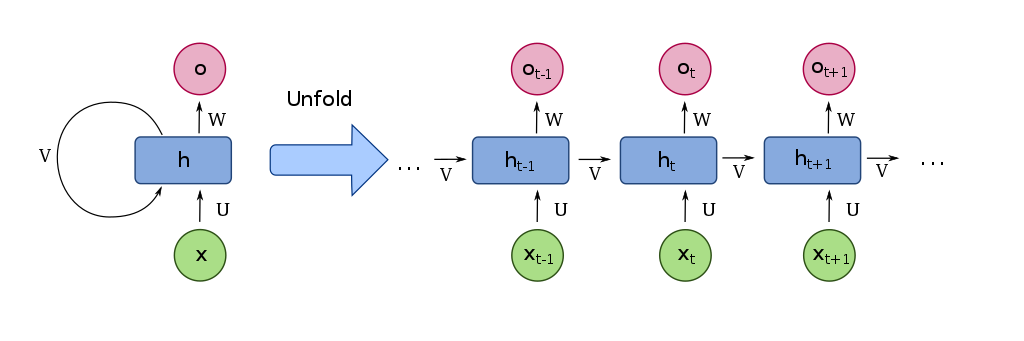
\includegraphics[width=\textwidth]{rnn-figure}
    \caption{A graphical representation of a RNN.\ The right image shows the
    model unfolded over a number of time steps. Source:~\cite{olah2015lstm}.
    }\label{fig:rnn}
\end{figure}

However, the standard RNN suffers from the problems of exponential decay or blow
up of error signals that are backpropagated through the network --- a situation
that only gets worse as the time dependencies increase
(~\cite{hochreiter2001gradient}). To remedy this, LSTM networks are used instead.

An LSTM network is composed of carefully designed memory cells containing
multiple special purpose weight matricies called gates, that determines what
information to remember, what to forget, what to do with the input and the
output of the network. In addition, a main state, $c$, of the network cell is
maintained and used to compute a hidden state, $h$, which is passed on to be
used at the next timestep, similar to the standard RNN.

The gates and states are calculated in the following manner
(~\cite{huang2015bidirectional}):\footnote{Note that
    these calculations are done by the respective frameworks we have been
working with and are not something, we have implemented ourselves}


\begin{align*}
    & i_{t} = \sigma(W_{xi}x_{t} + W_{hi}h_{t-1} + W_{ci}c_{t-1} + b_{i})    \\
    & f_{t} = \sigma(W_{xf}x_{t} + W_{hf}h_{t-1} + W_{cf}c_{t-1} + b_{f})    \\
    & o_{t} = \sigma(W_{xo}x_{t} + W_{ho}h_{t-1} + W_{co}c_{t-1} + b_{o})    \\ \\
    & c_{t} = f_{t}c_{t-1} + i_{t}\tanh(W_{xc}x_{t} + W_{hc}h_{t-1} + b_{c}) \\
    & h_{t} = o_{t}\tanh(c_{t})
\end{align*}

where $i_{t}$, $f_{t}$ and $o_{t}$ are the input gate, the forget gate and the
output gate respectively at time $t$, $c$ is the cell state and $h$ is the
hidden state. The weight matrices $W$ maps from either an input $x$ of size $m$
to an internal state or gate of size $n$ (ie. $W_{xf} \in \mathbb{R}^{m \times
n}$ is the input-forget gate matrix), or between two internal components (ie.
$W_{hi} \in \mathbb{R}^{n \times n}$ is the hidden-input gate matrix)
(~\cite{huang2015bidirectional}). A graphical representation of an LSTM Network
is given in Figure~\ref{fig:lstm}.

\begin{figure}[h]
    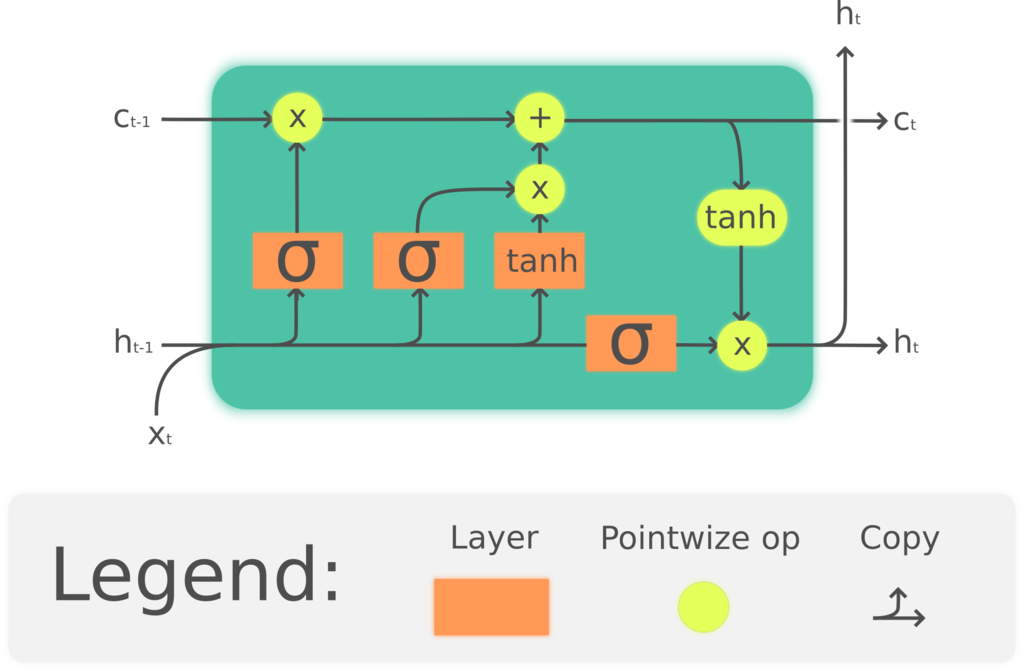
\includegraphics[width=\textwidth]{lstm-figure}
    \caption{A graphical representation of an LSTM unfolded. Source:~\cite{olah2015lstm}.
    }\label{fig:lstm}
\end{figure}

The activation function $\sigma$ is the sigmoid function, which squishes the
values of the gate matrices into the interval $[0,1]$. This means, that the
gates determine which and how much information is passed through and stored in
the memory cell. For example, the forget gate $f_{t}$ at timestep $t$ is
multiplied with the previous cell state $c_{t-1}$ to determine what to remember
and what to forget when $c_{t}$ is computed. A value of $1$ in the gate matrix
means `keep all' where a $0$ means `forget all'.\footnote{This particular forget
    mechanism was not introduced by Hochreiter in his original LSTM paper and,
    according to~\cite{pitis2016lstm}, `led the original [\ldots] model to have
    trouble with simple tasks involving long sequences'. This solution was
    introduced by~\cite{gers1999learning} and is now standard in LSTM
implementations.}

Updating the cell state also entails adding the element wise product of the
input gate $i_{t}$ and \textit{the candidate write} given by $\tanh(W_{xc}x_{t}
+ W_{hc}h_{t-1} + b_{c})$. Since the hidden state $h_{t} = o_{t}\tanh(c_{t})$
the candidate write at timestep $t$ consists of not only the weighted current
input $W_{xc}x_{t}$ but also the weighted result of passing the previous cell
state through the previous output gate $W_{hc}h_{t-1}$ where $h_{t-1} =
o_{t-1}\tanh(c_{t-1})$.

In other words, the memory cell at timestep $t-1$ produces a reading of its own
cell state which it passes on as a hidden state to the memory cell at timestep
$t$ to be used to compute the candidate write for $c_{t}$. For further
discussion of this somewhat reversed read/write procedure, refer
to~\cite{pitis2016lstm}.

The intricate design of the LSTM memory cell allows for time dependencies
spanning very long sequences through careful regulation of the cell state.
Applying a separate LSTM network layer that processes the same sequence of data
but in reversed order, the model becomes bidirectional. This means, that the
model can also use information from `the future' (ie.\ at later timesteps) to
infer knowledge about input at the current timestep.

However, at each timestep $t$ there will be two memory cells: one for the
forward pass and one for the backward pass. The first will depend on all $x_{i}
\in \{x_{0}, \ldots, x_{t-1}\}$ where the second will depend on all $x_{j} \in
\{x_{t+1}, \ldots, x_{T}\}$. This requires that the entire sequence of data is
provided before an output can be produced, but at the same time it enables the
output to be computed taking both past and future dependencies into
consideration.


\subsubsection{CRF}

When performing sequence labelling as we do in part-of-speech tagging and named
entity recognition, we want to predict a sequence of output tags $\bm{y} \in
\mathbb{R}^{K}$, where $K$ is the sequence length, given a sequence of input
features $\bm{X} \in \mathbb{R}^{K \times C}$ where $C$ is the number of
possible classes each tag can take.

The Conditional Random Field model (CRF) provides a method for computing the
probability of an output sequence $\bm{y}$ given an input sequence $\bm{X}$
under the assumption, that there exists conditional dependencies for
transitioning between any two $y_{k}$ and $y_{k+1}$ where $k \leq K$.

For example, in named entity recognition we work with tags such as `O', `B-PER'
and `I-PER', which classify words as non-entities (`O', eg.\ `Hello'), the first
part of a person entity (`B-PER', eg.\ `Claus') or a word inside a person entity
(`I-PER', eg.\ `Madsen'). Here, we assume that there is a higher probability of
transitioning from a tag `B-PER' to a tag `I-PER' than, say, from a tag `O' to a
tag `B-PER'.  That means, that the probability of tag $y_{k}$ being of some tag
type is conditioned on whatever $y_{k-1}$ was.

Knowing these transitioning scores, which will be the learnable parameters of
the CRF model, we can compute the conditional probability of specific sequence
of tags given an input sequence of feature vectors $p(\bm{y}|\bm{X})$.

The input sequence is often called the emission scores and that is what we will
use here onwards. The emission scores in our model comes from the feature
representation generated by the Bi-LSTM network after they have been passed
through the linear layer and mapped to tag space. 

For a regular classification problem, we could now compute $p(\bm{y}|\bm{X})$ by
taking the product of the probability of all $y_{k} \in \bm{y}$ and dividing it
by the normalization factor $Z(\bm{X}) = \prod_{k=1}^{K} Z(\bm{x}_{k})$ (also
known as the \textit{partition function}):

\begin{align*}
p(\bm{y}|\bm{X}) & = \prod_{k=1}^{K} \frac{\exp( W(\bm{x}_{k}, y_{k}) )} 
                                            {Z(\bm{x}_{k})} \\
                 & = \frac{\exp( \sum_{k=1}^{K} W(\bm{x}_k, y_{k}) )}
                                            {Z(\bm{X})}
\end{align*}

where $W(y_{k}, \bm{x}_{k})$ is the emission scores generated by the LSTM
network, here represented with a weight matrix $W$ to be consistent with general
notation (~\cite{treviso2019crf}).

For a conditional random field model however, we want to include the
dependency between label $y_{k-1}$ and $y_{k}$. This can be done by multiplying
with the probability of $y_{k}$ given $y_{k-1}$, ie. $p(y_{k}|y_{k-1})$. For
this, a transition matrix $T \in \mathbb{R}^{C \times C}$ is introduced, which 
is the trainable parameter of the CRF model:

\begin{equation*}
p(\bm{y}|\bm{X}) = \frac{\exp( \sum_{k=1}^{K} W(\bm{x}_k, y_{k}) +
                    \sum_{k=1}^{K-1} T(y_{k+1}, y_{k}) )}{Z(\bm{X})}
\end{equation*}

The challenge from here is to calculate the partition function $Z(\bm{X})$ as
this has to sum over all possible values of $y_{k}$ for all $1 \leq K$. This is
infeasable if implemented in a naive manner, but the whole crux of CRF is the
\textbf{forward} (or \textbf{backward}) algorithm, which enables the computation
to be done in time proportional to $O(CK^{2})$. A detailed description is out of
scope for this report, but is explained in great detail
in~\ref{sutton2012introduction}.

Performing inference using a CRF model (ie.\ predicting the most likely sequence
of tags $\bm{y^{*}} = \argmax_{y}p(\bm{y}|\bm{X})$) is done using the Viterbi
algorithm (~\ref{} something). This exploits the same recursive feature of the
model as the forward algorithm uncovers, and then stores backpointers to the
most likely tag $y^{*}$ at each time step $k$.

In short, our \texttt{Bi-LSTM-CRF} model is simply an extension of the
\texttt{Bi-LSTM} with an added CRF layer for modelling the conditional
dependencies between each successive tag in the sequence.

\subsubsection{Dropout layers}

The dropout layers are not part of the model besides training. Dropout is a
regularization technique which helps prevent the model from
overfitting~\cite{goodfellow2016deep}. Regularization is when we make changes to
reduce a models generalization error, ie.\ the errors on the test data, possibly
introducing more errors on the training data. Many different regularization
techniques exist and dropout is just one of these.

Dropout is about introducing variance in the model trained by randomly removing
output values. When thinking of the model as a network of neurons, dropout is
like randomly removing neurons from this network. What this means in relation to
the computational graph built, is that some of the elements in the vector output
of a node in the graph, is set to 0. To make up for randomly setting values to
0, some work has to be done. There are two different ways to handle this, one
which requires updating all other values in the output during training, and
another where we update the weights after training~\cite{goodfellow2016deep}.
Since this feature is common in every framework we used, we didn't have to
choose between one or the other method, and simply used the framework defaults.
In theory there shouldn't be any difference between the two different methods.

Dropout works by preventing the model from relying on specific element values in
the output of a layer. If the model is reliant on a single value, it would
completely fail when this value is set to zero, thus requiring it to learn a
different representation without this flaw. Another way~\ref{goodfellow2016deep}
of reasoning about dropout is to view it as an ensemple method. Ensemple methods
are about training different multiple networks and using their collective
results to best predict the correct values. Since dropout removes neurons from
the network for a single example, this is in a sense equivalent to training a
model without those neurons. A simple network of five neurons, two input, two
hidden, and one output neuron, could become 16 different networks. One extreme
being all five neurons remaining in the network, and the other extreme the
network consisting of only the output neuron. Since the number of networks
increase exponentially with the number of neurons in the network, not all of
these will be trained on, but depending on the dropout rate, some sample of the
networks will be used. This is different from ensemple methods since we only
have a single network, but since we are training on many different subsets of
the network, these subsets have been trained to solve the task without relying
on other parts of the network. 

We could have included dropout on the training input instead of just the output
of some of the layers. This would make sure the model trained on unknown as well
as known words. Since we are using a polyglot embedding for the input which
doesn't contain all words from our training data, we already do this to some
extend and we therefore decided against adding explicit dropout on this data as
well.

We picked a dropout rate of 50\% since this seems to be the generally agreed
upon be value for hidden layers in the model~\cite{}. If we had included dropout
on the input~\cite{} suggests that a dropout of 80\% is the best for this.


\subsubsection{Optimizer}

The optimizer is the algorithm used to update the weights and biases in the
network. After computing a loss by forward propogation of results, followed by
back-propogation to calculate the gradient, we need an algorithm to decide how
to update the network based on the gradient. The goto algorithm is the
stochastic gradient descent (SGD), not only is it simple, it also works very
well and competes against newer algorithms with more sofisticated ways to decide
how to update the network.

SGD updates based on a fixed learning rate. After calculating the gradient, the
update rule is to subtract the weights by the gradient scaled by the learning
rate. Using a fixed learning rate would suggest that the network can't converge
to a local minimum, and one would have to gradually decrease the value over
time. To our knowledge the frameworks used don't automatically implement any
kind of weight decay or momentum for the default SGD, this would have to be
manually specified. As such the models may not be able to converge to a local
minimum before they stop training.


\subsection{Configurations}

There are a total of 3780 different combinations of configurations based on the
7 parameters we decided to work with. 

A short list of the parameters are given below, and are explained more in detail
in the subsequent chapters.

%TODO: Make nice table or something
Frameworks: Dynet, PyTorch, TensorFlow

Languages: Arabic, Danish, Hindi, Japanese, Norwegian, Russian, Urdu

Tasks: Part-of-speech, Named Entity Recognition

Models: Bi-LSTM, Bi-LSTM-CRF

Seeds: 322233, 521403, 421213, 5123, 613321

Mini-batch-size: 1, 8, 32

Epochs: 1, 5, 50 using early stopping patience 3


\subsubsection{Languages}

The rationale behind the languages picked is a combination of word ordering,
language family and genus, availability of data, and the origin of the data.

The word ordering is the relative ordering of verbs, subjects, and objects (eg.\
verb-object-subject or VOS). We used~\ref{}{https://wals.info/chapter/81} to
determine the word ordering of languages and picked languages with one dominant
word ordering, ignoring languages such as German which has alternating word
orderings.

Language families are groupings of languages based on some common ancestral
language. Languages from the same family often share similarities such as word
orderings and some words. 

For word orderings with many languages to choose from, we picked two languages
from the same language family, and one language from a different family.
Language families were similarly based on~\ref{}{https://wals.info/languoid}. We
split languages based on both their family and genus, meaning a language such as
German (indo-european, germanic) is considered different from Italian
(indo-european, romance).

Sadly due to limited availability of pre-existing annotated datasets, we
couldn't find data on more than 3 different word orderings. For the more common
word orderings, subject-object-verb and subject-verb-object, there was a descent
range of languages to choose from. But for the less common word orderings we
could only find a single verb-subject-object language with enough data. There
was no data for the remaining languages. 

The 7 languages we picked, along with their word ordering, language family and
genus is given in~\ref{} below.

% TODO: Make nice table
* Arabic,   VSO, Afro-Asiatic, Semitic 

* Hindi,    SOV, Indo-European, Indic

* Urdu,     SOV, Indo-European, Indic

* Japanese, SOV, Japanese

* Danish,   SVO, Indo-European, Germanic

* Norwegian,SVO, Indo-European, Germanic

* Russian,  SVO, Indo-European, Slavic

The concern of availability of data and the origin is elaporated on
in~\ref{}{3.1}


\subsubsection{Model implementations}

All experiments have been conducted across three popular and open source machine
learning frameworks, two dynamic and one static. Each member of the project
group have had responsibility for the implementation of the models in one of the
frameworks. This section will briefly describe the experience and caveates with
working with each of the frameworks.

This subsection will give a descriptive introduction to each framework, how it
works and the implementation details relevant for this project. For a discussion
and evaluation of each framework, refer to Section~\ref{subsec:frameworks}.

\subsubsection*{A note on computational graphs}

% TODO: Move to relevant section
When describing neural networks the goto abstraction is that of neurons which
are linked to each other and arranged in layers. A neuron receives the output of
each neuron from the previous layer, computes its own value, and sends it to the
next layer alongside all the other neurons in its layer. Since it would be too
computationally expensive to calculate the result of each neuron individually
the neural network abstraction is discarded in favour of a matrix and vector
based representation which is closer to how the results are calculated in the
computer. The concept of layers however remains, so a simple layer could be
represented as the calculation $\sigma(W \cdot X + B)$, where $\sigma$ would be
the activation function sidmoid. 

\ref{Deep learning 6.5.1, NNM for NLP ???}

When neural networks are implemented in frameworks the layer abstraction is also
ignored in favor of so called computational graphs. In a computational graph
each node in the graph represents a single mathematical operation, or an input
value. As such the simple layer from before would be split into three distinct
nodes connected in succession. The values for $W$ and $X$ would be input into a
matrix multiplication node. The result of this node would be the input alongside
$B$ to a vector addition node, which would be the only input value to the
sigmoid node. 

Computational graphs as such don't provide much of an advantage over the layer
abstraction. Conceptionally we are still doing the same mathematical operations
on the input the performance of this model is not better than the layer based
representation, since we are still taking advantage of the same performance
gains from doing working with vectors and matricies. The reason behind the use
of computational graphs is because it simplifies calculating the gradients of
the network through the backpropagation algorithm. 

The backpropagation algorithm uses the chain rule of derivatives to calculate
the derivative of input values wherever they may be in the computational graph.
Since the chain rules is used for computing the derivative of arbitrarily many
functions, and computational graphs represents each function by its own node,
the graph abstraction simplifies calculating derivatives since each node only
needs to know the rules for computing the derivate of itself.
 

\subsubsection*{DyNet}

DyNet is an open source dynamic neural network framework developed by Garnegie
Mellon University and many others \ref{https://github.com/clab/dynet}. The
framework being dynamic means the computational graphs are recreated for each
input. This is particularly useful for natural language processing where
sentences don't have a fixed length so the unique structure of each sentence's
graph can be made without having to add padding to match the longest sentence in
the dataset. A downside of dynamic frameworks is that they are generally slower
than their static counterparts, the creators of DyNet though mention that it
performs comparable or faster than similar static declaration
frameworks~\ref{https://arxiv.org/pdf/1701.03980.pdf}.   

DyNet further allows for what they call auto-batching which means that sentences
don't have to be manually batched when training on batches of
sentences~\ref{On-the-fly Operation Batching in Dynamic Computation Graphs}. In
other frameworks, dynamic or not, users have to add a dimension to their input
which represents the batches. In DyNet this can be done by implicitly creating a
graph for each input in the batch and aggregating the losses, creating a
combined computational graph, which can be optimized to run parts in parallel.
The DyNet implementation aggregated using the sum of the losses, however this
was not possible for the other frameworks due to what we suspect was overflow
errors, which wasn't experienced in DyNet. 

A consequence of the framework being dynamic is that the structure of the model
is mixed with the processing and training on input. The model parameters are
defined by themselves, but since the input is an integral part of the
computation graph, the structure is defined by the mathematical operations
performed on the specific input values instead of a more general structure which
works on any input. This only has an impact on the structure of the source code,
and in extension how easy it is to understand it. The input should be processed
in the same way as it would be in a static framework, assuming the same
structure has been defined. This also means that instead of thinking of the
model as layers it is often better to think about the underlying operations of
the layers. The exception is the LSTM layer where much of the
implementation detail has been hidden behind a concise interface.

For training the \code{SimpleSGDTrainer} was used. For the embedding layer, the
polyglot embedding was converted to could be used to initialize a
\code{LookupParameter}. The Bi-LSTM was implemented using the
\code{LSTMBuilder}, and the \code{BiRNNBuilder}. Dropout could be implemented
using the \code{dropout} method. Early stopping was implemented by saving the
currently best seen model each time the model was improved upon. This creates
some overhead, but nothing noticable. If no improvements were seen for three
epochs, the model was loaded and training terminated.

DyNet doesn't have a CRF layer implemented as part of their library so we based
our implementation on the work of~\ref{Barbara}, which in turn based parts of
theirs on~\ref{Someone else, see their source code}. 

Due to miscomunication the DyNet model used two Bi-LSTM layers, this gives has
been shown to give better accuracy at the cost of longer training times. We
decided to prefer the shorter training over the better accuracy, but didn't make
this clear. As a result, we would expect DyNet to perform better in the
experiments.

% TODO: Move to environment?
DyNet doesn't support multi-threading in their python implementation as of the
time of this report, so all the experiments were run on a single core. 

\subsubsection*{PyTorch}

PyTorch is an open source, dynamic deep learning toolkit build on top of Torch
and developed by the Facebook research team (~\ref{}
\url{https://www.infoworld.com/article/3159120/facebook-brings-gpu-powered-machine-learning-to-python.html}).
PyTorch provides a \code{tensor} object, that is nearly identical to NumPys
\code{ndarray} but has two important advantages:

\begin{itemize}
    \item It allows for seamless computation through the GPU instead of the CPU
    \item It records the computational graph on the fly, allowing for easy
        backpropagation
\end{itemize}

As opposed to DyNet, PyTorch does not have any auto-batching feature. It does
support mini-batches through its API and most of its models and functions accept
a \code{batch\_first} argument where relevant, which indicate whether the first
dimension of the input corresponds to the batch size or not.

However, batching is rather poorly described by the documenation of the
framework, and there seem to be only sparse official description of how
mini-batches are expected to be arranged\footnote{\url{https://towardsdatascience.com/taming-lstms-variable-sized-mini-batches-and-why-pytorch-is-good-for-your-health-61d35642972e}}.
As an example, working with sequential data of variable length (such as
sentences), each input element has to padded so as to make the lengths uniform.
This may be common knowledge to an experienced ML researcher, but neither the
PyTorch documentation or official tutorials (at least not under the topic of
NLP) touch on this aspect.

Furthermore, to handle these batches of inputs of variable lengths, some modules
require the client to pass a masking tensor as argument (ie.\ a matrix of ones
and zeroes) to mask out padded values. Most ill-explained, however, is using
mini-batches together with the \code{LSTM} layer provided by the framework
itself. Here, it is necessary to pass the mini-batch of padded input sequences
(ordered by original sequence length in descending order) through
\code{pack\_padded\_sequence} function provided by the \code{torch.nn.utils.rnn}
module together with a list of the original lengths of each sequence. This
transforms the input so it can be handled properly by the \code{LSTM} layer, but
afterwards it has to be unpacked again using \code{pad\_packed\_sequence}. Not
only is this a rather intricate API, it is also only sparsely documented
considering how normal an operation training on mini-batches is.

As for the actual implementation of the two models in PyTorch, as much
pre-existing code within the framework as possible was used. This includes the
\code{Embedding}, \code{Dropout}, \code{LSTM} and \code{Linear} layer (all
provided through the \code{torch.nn} module), aswell as the
\code{CrossEntropyLoss} function for calculating the loss on the
\texttt{Bi-LSTM} model. The general structure of the model, the training
function and the evaluation function were created from tutorials, examples and
existing applications.\footnote{\url{https://pytorch.org/tutorials/beginner/nlp/sequence_models_tutorial.html}}\footnote{\url{https://github.com/jiesutd/NCRFpp}}\footnote{\url{https://github.com/pytorch/examples}}

The CRF layer was implemented using the existing PyPi package
\texttt{pytorch-crf} (v.0.7.2) by Kemal Kurniawan under the MIT
license.\footnote{\url{https://github.com/kmkurn/pytorch-crf}}

\textit{Early stopping does not save the best model, but returns the third one
after it}
\textit{Batching ignores remaining data, when it is not evenly dividable with the
batch size}


\subsubsection*{TensorFlow}
TensorFlow is an open source static deep learning framework developed primarily
by Google. Keras is a high-level API for frameworks like TensorFlow, CNTK and
Theano.

A significant effort has been spent to align TensorFlow with Keras, so much so
that it is sometimes hard to tell if you are dealing with pure TensorFlow
functionality or a Keras API\@. This topic is expanded on in Section~\ref{TODO}.

As such our implementation is based on Keras with TensorFlow as its
backend.

While the API allows manual control over how batching is done, it defaults to
just handling batching automatically.

Because the framework is static padding the input data is required, however
since we are using recurrent neural networks we can deal with dynamically sized
input. We do this by setting a mask value in the RNN layer to the padding
value, as such the padding should not affect the quality of the training.

LSTM is implemented using the implementation provided by Keras.
The CRF implementation is based upon a CRF layer by
Hironsan.\footnote{\url{https://github.com/Hironsan/keras-crf-layer}}

\subsubsection{Experimental setup}

For all languages, frameworks, and tasks we ran experiments on three different
mini-batch sizes, three epoch settings, and with five seeds. Additional
consideration were also made in regards to the training data to make for as fair
comparisons as possible.

The three mini-batch sizes were motivated by~\ref{Reymer and gurevych} who
reported worse accuracy for larger sizes of mini-batches with a sweet spot
between 8 and 32. Similar low values are used by
\ref{https://arxiv.org/pdf/1508.01991.pdf}. While this emperically seems to
work, it is a bit counter to the theory. Ideally we would train on the whole
training set to get the most accurate loss values, which would in turn allow us
to make the optimal update to the model to reduce the loss. We don't have to use
the whole training set and can do fine with an estimate of the true loss by
using mini-batches, however we would still expect bigger mini-batch sizes to
improve the estimate and result in better, but slower training \ref{Deep
Learning}. 

The fact that bigger mini-batch sizes leads to worse results, suggests that a
better estimate is not necessarily better for training. While a better estimate
of the true loss results in a more optimal update to lower the loss, the greater
variance in the loss estimate can also work as a regularization technique which
results in better generalization ~\ref{Deep Learning}. The lower mini-batch
sizes can then be explained as a way to avoid the model from getting stuck in
local minima.

The three epochs is to see how well the models perform based on very limited
training, on some reasonable amount of training, and the upper limits of the
models for the tasks. The expectation is that a single epoch of training gives
very bad performance on the tasks. Five epochs is the baseline where we expect
that none of the models have begun overfitting, while still able to produce some
reasonable predictive power. The last epoch setting is early stopping with a
patience of three, and a max of 50 epochs. This means that the model continues
training intill it has made three updates, which didn't improve the accuracy on
the validation set. Early testing suggests that models stopped improving before
the max, so we expect this setting to reasonable represents the best of what the
models can achieve. It is possible that with a lot more training, or different
hyperparameters, that the models can get an even better performance than our
early stopping allows.

The different seeds are used to get a better idea of the performance of the
models than a single run would give. This approach is based on the work
of~\ref{Reimers+Gurevych, misconceptions in nsl yang zhang} who demonstrated how
a single result comparison between two models is insufficient when randomness is
involved. If one model performs better than average on a run, and another model
performs worse than average, this might suggest that the model which performed
better is a better model. But if more runs are used it is possible to compare
the average, minimum and maximum accuracy of models, along with the standard
deviation to give a better perspective on the relative performance of the
models. This helps mitigate situations where we mistakenly conclude that one
model is better than another.

To make comparisons between languages more fair, we limited the data on the
number of sentences for training, testing, and validation. The cutoff made was
5000 sentences, where 4000 is used for training and the last 1000 was split
evenly between validation and testing. The numbers picked were based on
availability of data with a preference for more sentences. From the datasets,
the first 4000 sentences were used for training, next 500 for validation, and
next 500 for testing. Any remaining sentences in the data were discarded.

Due to the nature of the languages each training set might contain a differing
number of words in each sentence, we didn't do anything to equalize this since
the word count wouldn't affect the number of updates when training. There is a
risk that since the language would also be tested on longer sentences, and we
may assume it is harder to correctly label longer sentences than shorter ones,
the accuracy might be lower for these languages than others. The languages with
longer sentences in their test set however is most likely also the languages
with longer sentences in their training set this hopefully evens out the
mistakes.

The datasets found are created from different types of sources, eg.\ news, blog
posts, reviews, etc. We wanted the datasets for the different languages to be
created from similar sources. It was infeasible to find datasets for both tasks
which were created from similar sources, but within each task, the data is to
some degree made from the same kind of source, the details are included in their
respective chapters.

There was an issue in the japanese dataset where we ignored a lot of the tokens used.
The size of our training sets are relatively small. The Penn Wall Streets
journal treebank \ref{https://catalog.ldc.upenn.edu/LDC95T7} often used for the
part of speech task, contains over 1.6 million words, where our datasets,
depending on the language, contain around than 100.000 words split over
training, testing, and validation files. As more data generally improves the
accuracy of the models we would expect our models to do worse than models
trained on a larger dataset, assuming similar network structure. The size is
however not too small to learn a good representation.
\ref{https://www.aclweb.org/anthology/P16-2067} found, when comparing the
accuracy of different types of taggers, that when training on as little as 1000
sentences their model could get over 90\% accuracy on a wide range of languages.

% TODO: Extra notes

The datasets from the different tasks were standardizes such that there was no
need for task specific code. 

We used the polyglot package to load the word embeddings. Specifically the
Embeddings class from polyglot mappings library. 
There are a lot of different polyglot embedding 


\pagebreak

\subsection{Machine environment}

The experiments were executed across several AWS EC2 machines, as they offer
quite powerful virtual machines.

\subsubsection{Detailed description of machine environemnt}

The experiments ran concurrently in their own process with multithreading
turned on for the frameworks that supported it. The experiments ran on a
mixture of instances of type \texttt{c5.9xlarge} and
\texttt{c5.18xlarge}.\footnote{For the difference between instance types see
\url{https://aws.amazon.com/ec2/instance-types/}}
Each machine had a 32 GiB magnetic harddisk attached as its primary storage.
The key difference between the machines was the vCPU count, the memory
difference had no impact on execution.

Each machine ran software with the following versions:
\begin{itemize}
  \item{Ubuntu 18.04.2 LTS}
  \item{Python 3.6.7}
  \begin{itemize}
    \item{NumPy 1.16.2}
    \item{Keras 2.2.4 / TensorFlow 1.13.1}
    \item{dyNET 2.1}
    \item{PyTorch 1.0.1.post2}
  \end{itemize}
\end{itemize}

For dynet 34 processes were executed concurrently depending on the
instance type.
For tensorflow 5 processes were executed concurrently.
Pytorch initally ran 2 processes concurrently with multithreading enabled, but
was changed to 34 processes with multithreading disabled midway through the
execution of the experiments.

\subsubsection{Differences between AWS and development environment}

Notable differences between execution in the development environment and on the
EC2 servers were noticed and are summarised by the following:

Pytorch grinded to a halt on the 36 core EC2 machine. Switching to a 72 core EC2
machine without disabling multithreading only exacerbated the problem. It turns
out that pytorch's multithreading does not support a high amount of
cores\footnote{As evidenced in this Github issue \url{https://github.com/pytorch/pytorch/issues/9873}}.

Tensorflow had no noticable differences between the development environment and
the EC2 machines.

Some dynet configurations took more than six times the time to complete on an
EC2 machine compared to the local development environment. The exact cause is
not known to us.

\subsubsection{Comparability of speed results}

Given the complications stated in the above sections, none of the speed results
are truly comparable. This a result of several factors.
One being that 2 different EC2 instance types was used, where one was faster
than the other, or in pytorch's case slower.
Another is the fact that each experiment was run concurrently with others. This
would have only had a minor impact, if multithreading had not been enabled for
some of the frameworks.
Lastly dynet behaved unexpectedly with regards to execution time, compared to the
development environment.

Ideally each experiment would be run one at a time, or with multithreading
disabled, on identical EC2 machines. Seeing as that was not the case, no
conclusions can be made with regards to the speed of the frameworks, only hints
at where further experimentation with tighter control might be warranted.
% Here we could add something about master/slave pattern og maybe how utilising
% AWS Batch would have been "oplagt", sorta, tror ogsaa det ville have vaeret
% lidt besvaerligt :/


\pagebreak


\section{Experiments}


\subsection{Part-of-speech tagging}

This section will go into the details of the Part-of-speech task, what the
specifics are, considerations in regards to the data used, any issues we came
across, and the results of our experiments.

\subsubsection{Task definition}

The Part-of-Speech task is a classification task where the objective is to label
each word in a sentence with it's corresponding part-of-speech label such as
noun, verb, adjective, etc. Some languages have more of labels than other. The
same words can have different labels in different context, so the classifier
should be able to figure out the which label is a better fit on a sentence by
sentence basis. Simply remembering that word $X$ has label $Y$ wouldn't be able
to generalize very well.

The performance of a classifier for the POS task is the simple accuracy of the
predictions. Since there are no label which is a lot more common than others
guessing randomly would very rarely give a better accuracy than perhaps 10\%.

\subsubsection{Data}

For this task we used datasets from~\ref{}{UniversalDependencies.org} which has
a broad selection of languages with multiple datasets (called treebanks) in
each. The datasets from~\ref{}{UniversalDependencies.org} are all in the CoNNL-U
format, but are created from different types of sources. The source types are
given as tags such as news, legal, blog, wiki, etc.

Since the datasets from~\ref{}{UniversalDependencies.org} comes pre-split, these
were concatenated before splitting into our own sizes. Concatenation happened
using the command ``cat *.conllu > combined.conllu'', since the convention for
the datasets is to name the files something with train, test, and dev, the
assumed order of the files is dev, test, and train. Meaning that if the dev set
(eg. the validation set) contains 5000 sentence, only these were used in our
datasets, and none of the sentences from the test or training-sets would be
used. No guarantees however were made to guarantee this ordering, so depending
on the naming conventions used in the specific treebanks this might differ.

Some datasets, such as the Norwegian dataset, contains contractions as well as
the individual words. Since the contration is usually unlabelled in the datasets
these were simply removed from the data for ease of parsing. This has the
obvious consequence that the models are not trained on the contractions of words
which are often more commonly used, this however shouldn't affect the
comparisons between word orderings since contractions shouldn't affect these.

The treebanks we selected from~\ref{}{UniversalDependencies.org} were all made
from news, where some used additional sources such as non-fiction and spoken. A
list of the languages, their respective treebank selected, and their tags is
given below.

* Arabic,   PADT, news

* Hindi,    HDTB, news

* Urdu,     UDTB, news

* Japanese, GSD, blog, news

* Danish,   DDT, fiction, news, non-fiction, spoken

* Norwegian,Bokmaal, blog, news, non-fiction

* Russian,  SynTagRus, fiction, news, non-fiction

The distribution of tokens, labels, etc. is given in appendix.

\subsubsection{Results and analysis}


\pagebreak


\subsection{Named Entity Recognition}

This section will go into the details of the Named Entity Recognition task, what
the specifics are, considerations in regards to the data used, any issues we
came across, and the results of our experiments.

\subsubsection{Task definition}

Named Entity Recognition is a classification task of different types of
entities, such as places, people, organisation, times, and more. Entities can
consist of one or more words (and/or numbers), eg.\ ``Eurovision Song Contest
2019'' is a single entity of 3 words and a number. The classifier should
correctly identify the whole entity and not just part of it. We didn't take this
into consideration before running the experiments so our results are on a word
by word basis and doesn't tell us if the whole entity was correctly classified
or not.

The same entity might never show up in the dataset twice so it's important for
the classifier to be able to figure out based on context of the other words in
the sentence if there is an entity or not. It is impossible to simply remember
that a word refers to an entity since the word was most likely not seen during
training.

Usually the performance of a classifier for the NER task is measured by a $F_1$
Score, which considers the classifier's precision and recall. The precision is
the classifier's ability to correctly classify an entity given all attempts, and
recall is the ability to correctly classify an element given how many elements
exists. Say there are 100 entities in a document, the classifier finds 90
entities, 80 of them are correct, 10 of them are wrong, and 20 were not found.
From this we get the precision $P = {80 \over 80 + 10} = 0.88\ldots$, and recall
$R = {80 \over 80 + 20} = 0.8$. The $F_1$ score is simply the harmonic mean
between the precision and recall given by $F_1 = 2 \cdot {precision \cdot recall
\over precision + recall}$. Based on our example this would be $F_1 = 2 \cdot
{0.88 \ldots \cdot 0.8 \over 0.88\ldots + 0.8} = 0.8421$ \cite{f-measure}.

The rationale behind using the $F_1$ score is that usually a lot of the data is
non-entities. A classifier which classified nothing as an entity would have a
great accuracy on datasets with few entities. Since we didn't evaluate if whole
entities were classified correctly, we will base our score on the individual
words and the score might therefore be higher than otherwise. Since we aren't
comparing with models outside our own this shouldn't be an issue.

The reason the NER task is relevant is its usefulness in handling huge data
sizes, since the task is inherently about extracting information from text.
Extracting entities from a text would allow for easy tagging, comparisons
between documents, and linking to a knowledge base. A document mentioning
different locations and capital cities such as ``France'', ``Tokyo'', and ``New
Zealand'', could be about geografi or traveling. And similar a document
mentioning people associated with economy could be about economy
\cite{sang2003introduction}.

The state of the art model for NER based off of \cite{ner-state} is
\cite{baevski2019cloze}. They use a bidirectional self-attention cloze model
which seems very disimilar to anything we are doing. They achieve an F1 score of
93.5 on the CoNLL 2003 English dataset, which is 0.41 points above the previous
state of the art by \cite{akbik2018coling}, the same model mentioned in the
previous section with state of the art results for POS.

\subsubsection{Data}\label{sec:experiments-ner-data}

For the NER task we used auto-annotated wikipedia data from
\cite{pan-etal-2017-cross}. This dataset contains annotated data for 282
languages in varying sizes. 

The datasets are all in the BIO (or IOB) format, which has three different
entities; organisations, people, and locations. The BIO format uses the
convention that the beginning of an entity is prefixes with a B and the
continuation of an entity is prefixed with an I (for inside). Tokens which are
not part of an entity is labeled O (for other). This gives the 7 labels, B-ORG,
B-PER, B-LOC, I-ORG, I-PER, I-LOC, and O. 

Since all the datasets were created based on wikipedia data we didn't have to
take varying sources into considerations, as was necessary for the POS task.

The data being auto-annotated means it might not be of the same standard as the
POS data. Ideally this shouldn't affect the experiments since the word orderings
are still the same, and systematic errors in the data would hopefully happen for
all languages in the datasets.

For Japanese which doesn't use spaces to differentiate between the beginning and
the end of words, the data is split and labeled character by character, this
differs from the POS data where words are split in a more natural way. This has
an influence on the results and means that Japanese isn't as comparable between
tasks as other languages. Since it turns out that our Polyglot embedding has a
somewhat similar way to split words it can have a positive effect on the
performance.

Another issue with the Japanese NER dataset we used is that we ignored many of
the tokens in the dataset by mistake. For the CoNLL-U datasets, the \# symbol is
used for comments. When reading the datasets we simply skipped files starting
with the \# symbol and continued reading normally. This is only an issue for the
Japanese dataset since it was the only one using these symbols, however these
symbols constitudes around 5\% of the data. This is another issue with the
Japanese dataset, and it's hard to say if ignoring these symbols is beneficial
to the experiment or not.

As the data used for training the model is the same data used for training the
polyglot word embeddings, the models don't have the same kind of variety from
the data as is the case for the POS task. This may result in worse performance
since the models might be more likely to overfit.

A table of the languages with the number of entities in their respective dataset
is given below in Table~\ref{table:token-distribution-ner}. 

\begin{table}[h!]
    \centering
    \begin{tabular}{l c c c c c c c c c}
        \toprule
        \multicolumn{10}{l}{\bfseries Training} \\
        Language & Tokens & Distinct &
        B-PER & I-PER & B-LOC & I-LOC & B-ORG & I-ORG & O \\
        
        \cmidrule(lr){1-10}

        ar   &  27159 &  8567 &
        1929 &   3919 &  1835 &  2526 & 1112 &  2237 & 13601 \\

        da   &  35498 & 10247 &
        1419 &   1802 &  3385 &   991 &  974 &  1264 & 25663 \\

        hi   &  23276 &  4667 &
        3502 &   4021 &   700 &   830 & 1105 &  2943 & 10175 \\

        ja   & 122377 &  2429 &
        1644 &   6853 &  1663 &  4420 & 2575 & 10970 & 94252 \\

        no   &  41172 & 10988 &
        1525 &   2076 &  3229 &   943 & 1302 &  1506 & 30591 \\

        ru   &  26232 &  9817 &
        2483 &   5341 &   973 &   711 & 1109 &  2269 & 13346 \\

        ur   &  21391 &  3048 &
         502 &   1549 &   3012 & 10024 & 527 &  1500 &  4177 \\

        \cmidrule(lr){1-10}
        \multicolumn{10}{l}{\bfseries Testing} \\
        Language & Tokens & Distinct &
        B-PER & I-PER & B-LOC & I-LOC & B-ORG & I-ORG & O \\
        
        \cmidrule(lr){1-10}

        ar  & 2991 & 1039 &
         91 &  211 &  230 &  525 &  237 &  652 & 1045 \\

        da  & 4523 & 1682 &
        248 &  352 &  333 &  191 &  138 &  255 & 3006 \\

        hi  & 2884 & 1234 &
        180 &  288 &  110 &  177 &  268 &  892 &  969 \\

        ja  &14723 & 1176 &
        299 & 1730 &  155 &  471 &  229 & 1342 &10497 \\

        no  & 5574 & 1549 &
         25 &   31 &  492 &   65 &  155 &  243 & 4563 \\

        ru  & 2280 &  989 &
        456 & 1095 &   31 &   15 &   33 &   60 &  590 \\

        ur  & 2813 &  310 &
          0 &    0 &  487 & 1745 &   19 &   62 &  500 \\
        \bottomrule
    \end{tabular}
    \caption{Distribution of tokens on the NER data sets for each language.
    }\label{table:token-distribution-ner}
\end{table}

\subsubsection{Model comparison}

Starting by looking at number of epochs trained
(Table~\ref{table:epochs-run-ner}), we see that all models terminated training
some time before hitting the upper bound, with the TensorFlow implementation of
\texttt{Bi-LSTM} with a batch size of 8 being the slowest to converge (36.8
epochs on average). Also, we see that \texttt{Bi-LSTM-CRF} models converged
faster for most every batch size and implementation.

\begin{table}[h!]
    \centering
    \begin{tabular}{l c c c|c c c}
        \toprule
        \multirow{2}{*}{\bfseries Batch size}     &
        \multicolumn{3}{c}{\bfseries Bi-LSTM}     &
        \multicolumn{3}{c}{\bfseries Bi-LSTM-CRF} \\
        \cmidrule(lr){2-7}
        & DyNet & PyTorch & TensorFlow
        & DyNet & PyTorch & TensorFlow \\
        \cmidrule(lr){1-7}
         1 &  9.49 & 13.43 & 21.00 &  8.14 &  7.66 &  6.43 \\
         8 &  9.86 & 22.43 & 36.80 &  9.97 & 11.46 &  8.69 \\
        32 & 12.57 & 29.06 & 31.51 & 11.57 & 14.63 & 10.91 \\
        \bottomrule
    \end{tabular}
    \caption{Average of epochs run across all seeds and languages when trained
        with early stopping.
        }\label{table:epochs-run-ner}
\end{table}

However, when turning our attention to the \textit{F1} scores
(Table~\ref{table:f1-total-ner}), the models are performing very poorly, which
does not fit with the expected results of a well converged model. We suspect the
main reason for this, is the fact that our models did the same \textit{accuracy}
test during training to decide when to stop as was done in the POS task. But
since we for the NER task want to optimize our \textit{F1} score, the accuracy
test is really not the optimal parameter to use in early stopping --- it would
of course had made more sense to test if the \textit{F1} score had stopped
improving.

% F1 SCORE
\begin{table}[h!]
    \centering
    \begin{tabular}{c l c c c|c c c}
        \toprule
        \multirow{2}{*}{\bfseries Language} &
        \multirow{2}{*}{\bfseries Batch size} &
        \multicolumn{3}{c}{\bfseries Bi-LSTM} &
        \multicolumn{3}{c}{\bfseries Bi-LSTM-CRF} \\
        \cmidrule(lr){3-8}
        && DyNet & PyTorch & Tensorflow & DyNet & PyTorch & Tensorflow \\

        \cmidrule(lr){1-8}
        \multirow{3}{*}{\bfseries ar}
        &  1 & 
        \underline{\textbf{83.5}} & 78.6 & 74.3 &
        82.6 & \underline{78.7} & \underline{75.0} \\
        &  8 & 
        \underline{\textbf{82.4}} & 62.5 & 47.4 &
        80.8 & \underline{77.3} & \underline{66.2} \\
        & 32 & 
        79.2 & 42.4 & 27.8 &
        \underline{\textbf{79.3}} & \underline{70.0} & \underline{48.9} \\

        \cmidrule(lr){1-8}
        \multirow{3}{*}{\bfseries da}
        &  1 &
        \underline{\textbf{77.0}} & 70.5 & \underline{54.0} &
        76.9 & \underline{71.8} & 49.9 \\
        &  8 &
        \underline{\textbf{74.9}} & 48.1 & 23.5 &
        74.6 & \underline{69.3} & \underline{35.1} \\
        & 32 &
        68.0 & 27.7 &  0.0 &
        \underline{\textbf{69.2}} & \underline{61.4} & \underline{20.8} \\

        \cmidrule(lr){1-8}
        \multirow{3}{*}{\bfseries hi}
        &  1 &
        \underline{\textbf{69.7}} & \underline{65.3} & 52.2 &
        69.4 & 62.8 & \underline{55.5} \\
        &  8 &
        \underline{\textbf{68.3}} & 55.1 & 26.2 &
        67.3 & \underline{63.4} & \underline{51.2} \\
        & 32 &
        \underline{\textbf{64.0}} & 33.6 &  1.2 &
        62.6 & \underline{56.9} & \underline{37.9} \\

        \cmidrule(lr){1-8}
        \multirow{3}{*}{\bfseries ja}
        &  1 &
        \underline{\textbf{58.1}} & \underline{34.9} & \underline{35.4} &
        52.6 &  8.1 & 14.8 \\
        &  8 &
        \underline{\textbf{54.3}} & \underline{24.9} & 13.6 &
        47.6 & 11.7 & \underline{47.3} \\
        & 32 &
        \underline{\textbf{47.9}} & 22.5 &  9.3 &
        44.5 & \underline{27.8} & \underline{45.2} \\

        \cmidrule(lr){1-8}
        \multirow{3}{*}{\bfseries no}
        &  1 &
        65.2 & \underline{49.7} & 29.9 &
        \underline{\textbf{67.1}} & 44.5 & \underline{47.1} \\
        &  8 &
        \underline{\textbf{63.2}} & 25.4 & \underline{11.8} &
        61.4 & \underline{48.1} &  3.4 \\
        & 32 &
        \underline{\textbf{56.0}} & 18.2 &  \underline{8.3 }&
        50.1 & \underline{37.2} &  2.2 \\

        \cmidrule(lr){1-8}
        \multirow{3}{*}{\bfseries ru}
        &  1 &
        \underline{\textbf{96.6}} & 95.3 & 81.2 &
        96.6 & \underline{95.8} & \underline{93.3} \\
        &  8 &
        96.2 & 93.5 & 68.7 &
        \underline{\textbf{96.4}} & \underline{95.9} & \underline{93.0} \\
        & 32 &
        95.5 & 83.5 & 43.3 &
        \underline{\textbf{95.7}} & \underline{95.2} & \underline{87.2} \\

        \cmidrule(lr){1-8}
        \multirow{3}{*}{\bfseries ur}
        &  1 &
        \underline{97.8} & 96.8 & 95.2 &
        97.4 & \underline{\textbf{98.0}} & \underline{97.6} \\
        &  8 &
        \underline{\textbf{97.8}} & 93.6 & 82.9 &
        97.6 & \underline{97.7} & \underline{96.9} \\
        & 32 &
        96.3 & 84.5 & 71.1 &
        \underline{\textbf{97.4}} & \underline{96.5} & \underline{96.3} \\
        \bottomrule
    \end{tabular}
    \caption{F1 scores for NER experiments by language and batch
        size. Bold: highest accuracy for batch size plus language. Underline:
        highest accuracy for framework between \texttt{Bi-LSTM} and
        \texttt{Bi-LSTM-CRF}.
    }\label{table:f1-total-ner}
\end{table}


Furthermore, the loss function should also have been utilized differently. The
motivation for using the \textit{F1} score, is to focus attention on the models
ability to classify entities and not reward it too much for identifying
`O'-tokens. But for our cross-entropy loss, a true prediction of a tag `O' has
had the same influence as the true prediction of an entity tag. Since there are
a lot more non-entities than entities, it is reasonable to suggest, that the
models will have tuned their parameters to correctly classify non-entities and
accepted a lower accuracy rate for entity tags. This is also supported by the
results shown in Figure~\ref{chart:tag-acc-ner}.

\begin{figure}[h!]
    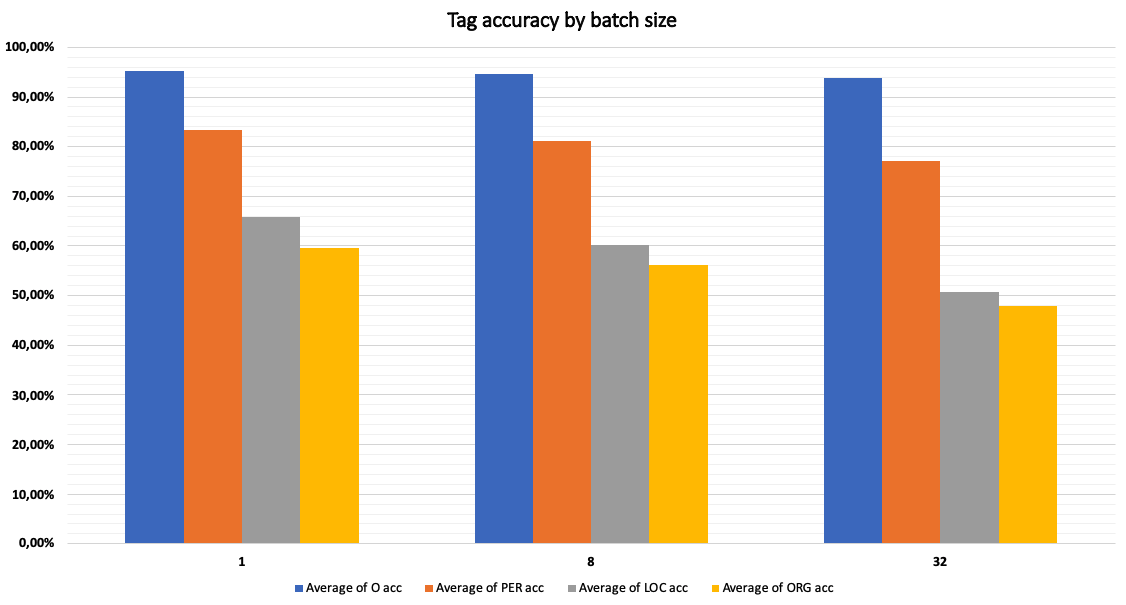
\includegraphics[width=\textwidth]{tag-acc-ner}
    \caption{Column diagram of averaged accuracy percentages for NER tags
        (B-<tag> and I-<tag> are combined in PER, LOC and ORG)
    }\label{chart:tag-acc-ner}
\end{figure}

Despite this design flaw, we still get some notable observations from the
obtained \texttt{F1} scores, depicted in
Figure~\ref{chart:f1-by-batch-and-lang}.  First of all, we once again see that
the DyNet implementations are by far the most succesfull, having the highest
score in all but one experiment. This is again attributed to its 2 layer
implementation of the bidirectional LSTM network. We also see the same pattern
as for POS, where the PyTorch implementation has the second best results and
the TensorFlow implementation is falling severely behind.

We also see, that the \texttt{Bi-LSTM-CRF} models in PyTorch and TensorFlow
outperforms their \texttt{Bi-LSTM} counterparts at almost every batch size and
language (the notable exceptions being cases for Japanese and Norwegian, where
the scores are extraordinarily low. See Section~\ref{sec:experiments-ner-data}
for more). This is interesting, as it confirms the expectation that the CRF
layer is able to significantly improve the performance in performing NER tasks
(~\cite{huang2015bidirectional}).

We still don't see a consistent improvement on the DyNet implementations from
the CRF layer. This again indicate, that the addition of a CRF layer to a 2
layer \texttt{Bi-LSTM} model is of negligible effect for these batch sizes.
However, we might see a small tendency for the larger batch sizes to benefit
from the CRF, as the DyNet \texttt{Bi-LSTM-CRF} model highest score in Arabic,
Danish, Russian and Urdu.

Another observation concerning applying CRF is how much it helps an increasing
batch size. For the pure \texttt{Bi-LSTM} models, a batch size of 32 drops the
performance by 36.4\% for the PyTorch implementation and by a whooping 61.9\%
for the TensorFlow implementation when compared to a batch size of 1. For the
\texttt{Bi-LSTM-CRF} models, these numbers go down to 3.2\% and 20.0\%
respectively. It should be noted, that the \textit{F1} scores for the DyNet
implementation actually experience a slight increase in the perfomance drop from
the larger batch size when CRF is applied (the drop goes from 7.5\% to 8.1\%).

\begin{figure}[h!]
    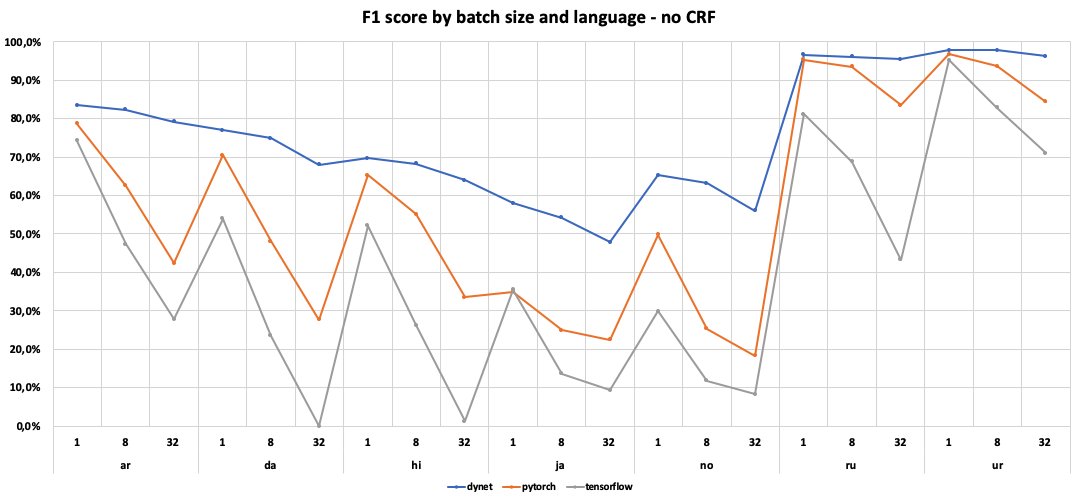
\includegraphics[width=\textwidth]{f1-no-crf}
    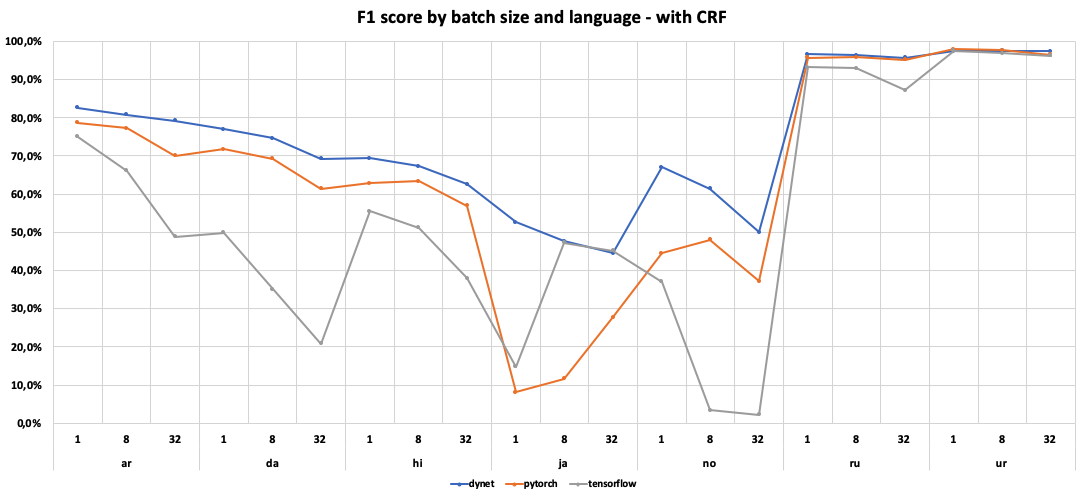
\includegraphics[width=\textwidth]{f1-with-crf}
    \caption{\textit{F1} scores for each framework implementation by batch size
        and language. Notice drops in performance when the batch size increases
        in models that does not utilize a CRF model. Top: the \texttt{Bi-LSTM}
        implementations. Bottom: the \texttt{Bi-LSTM-CRF} implemenations.
    }\label{chart:f1-by-batch-and-lang}
\end{figure}

\subsubsection{Language comparison}\label{sec:experiments-ner-lang-comparison}

Looking at the tag distributions in Table~\ref{table:token-distribution-ner}, we
notice several oddities, that are worth mentioning. As we consider the results,
we therefore first describe some potential problems related to the data, since
we believe they may be the cause of some of the strange values we get. The
results for each language are presented in Table~\ref{table:f1-total-ner} and
plottet in Figure~\ref{chart:f1-by-batch-and-lang}.

The training data for Norwegian looks reasonable when comparing with the other
languages, but for the test data there are very few entities (ie.\ non-`O'
tags). More than 80\% of the tokens are `O' tags which is noticably different
from the other languages. Since the \textit{F1} scores is calculated only on
entities, a large part of the test data is disregarded in this respect, and the
models \textit{F1} score will quickly be punished for misclassifications as each
prediction has a relatively higher weight compared to test data with more
entities.

Arguably the tagger should still be able to identify the entities correctly, no
matter how few there are. However, when looking at the results, we see
significantly lower scores than for most other languages. Adding the CRF layer,
we also observe that the PyTorch and TensorFlow models behave irregularly. For
the PyTorch implementation, the score improves by 3.6 when increasing the
batch size from 1 to 8, but then drops by 10.9 when it is increased to 32. For
TensorFlow, the score for a batch size of 1 is 47.1, but drops to 3.4 and 2.2
for batch size 8 and 32 respectively. In general, the increase in batch size
either leads to a steady decay or improvement of the scores (or only a very
small change one way or the other), so this behaviour is highly irregular.

Japanese has the second highest number of `O' tags which constitute slightly
above 70\% of the total test data. The results are not the same kind of
irregular as for Norwegian, but we do observe an unprecedented and sudden boost
in the perfomance of the TensorFlow \textit{Bi-LSTM-CRF} model over the others.
It especially seems odd, that this implementation --- that in all other cases
gets worse with an increasing batch size --- actually outperforms the
corresponding DyNet implementation at batch size 32. Further, as the only example
of this, the PyTorch \textit{Bi-LSTM-CRF} goes from 8.1 through 11.7 to 27.8 for
increasing batch sizes --- in all other cases, an increasing batch size for
PyTorch leads to decreasing scores. Last but not least, the Japanese scores are
overall by far the worst, so with these irregularities in mind aswell as the
data issues mentioned in Section~\ref{sec:experiments-ner-data}, we assume that
there are flaws in this experiment.

For Russian and Urdu, we observe that the test data almost solely consists of a
single entity type, which believe can make the results very inflated. For the
training data (and not counting `O' tags), Russian had 60.1\% person tags
(either `B-PER' or `I-PER') but for the test data, these tag types made up
91.8\% of the entity tags. For Urdu, the uneven distribution was even more
extreme: during training, 75.7\% of the entity tags were of type `B-LOC' or
`I-LOC' against a massive 96.5\% in the test data.

Add to that, that these two languages both have the lowest number of tokens and
the lowest number of distinct tokens. These facts may have an influence on why
the \textit{F1} scores for Russian and Urdu outperforms every other language.
All three framework implemenations achieve scores of more than 90\%, and the for
a batch size of 1, the PyTorch \texttt{Bi-LSTM-CRF} model reaches a stunning
score of 98.0.

\subsubsection*{Accuracy}

For completeness sake, we also include the data for our results on general
accuracy on the NER data in Table~\ref{table:acc-total-ner}. This was the actual
score our models trained to optimize and are as such relevant. 

Overall they align pretty well with the pattern found in the rest of the data,
but they are expectedly higher. The best results are generally either achieved
by the lowest batch size or by the \texttt{Bi-LSTM-CRF} and always by the DyNet
implementation. The best results reaches pretty impressive heights with
97.3\% for russian and 98.5\% for urdu. However since these accuracy scores can
get pretty high by just being really good at identifying non-entities, the
accuracy may not reflect the practical success of the models.

\begin{table}[h!]
    \centering
    \begin{tabular}{c l c c c|c c c}
        \toprule
        \multirow{2}{*}{\bfseries Language} &
        \multirow{2}{*}{\bfseries Batch size} &
        \multicolumn{3}{c}{\bfseries Bi-LSTM} &
        \multicolumn{3}{c}{\bfseries Bi-LSTM-CRF} \\
        \cmidrule(lr){3-8}
        && DyNet & PyTorch & Tensorflow & DyNet & PyTorch & Tensorflow \\

        \cmidrule(lr){1-8}
        \multirow{3}{*}{\bfseries ar}
        &  1 & 
        \underline{\textbf{88.4}} & \underline{87.4} & \underline{85.4} &
        88.3 & 84.1 & 81.6 \\
        &  8 & 
        \underline{\textbf{88.6}} & \underline{85.5} & \underline{81.1} &
        88.0 & 85.3 & 76.1 \\
        & 32 & 
        \underline{\textbf{88.9}} & 80.9 & \underline{77.0} &
        87.5 & \underline{84.8} & 71.5 \\

        \cmidrule(lr){1-8}
        \multirow{3}{*}{\bfseries da}
        &  1 &
        91.3 & \underline{90.5} & \underline{87.6} &
        \underline{\textbf{91.5}} & 89.8 & 81.6 \\
        &  8 &
        91.2 & 88.0 & \underline{85.3} &
        \underline{\textbf{91.2}} & \underline{90.4} & 75.8 \\
        & 32 &
        \underline{\textbf{91.1}} & 86.2 & 67.1 &
        91.1 & \underline{88.8} & \underline{74.2} \\

        \cmidrule(lr){1-8}
        \multirow{3}{*}{\bfseries hi}
        &  1 &
        \underline{\textbf{75.6}} & \underline{74.0} & \underline{72.0} &
        75.5 & 70.0 & 62.1 \\
        &  8 &
        74.6 & 71.5 & \underline{62.2} &
        \underline{\textbf{74.9}} & \underline{72.9} & 60.7 \\
        & 32 &
        74.3 & 64.8 & 34.4 &
        \underline{\textbf{74.5}} & \underline{70.1} & \underline{53.8} \\

        \cmidrule(lr){1-8}
        \multirow{3}{*}{\bfseries ja}
        &  1 &
        \underline{\textbf{83.7}} & \underline{80.0} & \underline{80.1} &
        81.4 & 52.2 & 72.8 \\
        &  8 &
        \underline{\textbf{82.4}} & \underline{80.5} & 77.8 &
        81.5 & 73.7 & \underline{79.4} \\
        & 32 &
        \underline{\textbf{82.1}} & \underline{79.4} & 77.1 &
        81.3 & 73.8 & \underline{81.0} \\

        \cmidrule(lr){1-8}
        \multirow{3}{*}{\bfseries no}
        &  1 &
        94.4 & \underline{86.4} & 87.2 &
        \underline{\textbf{94.4}} & 74.4 & \underline{87.3} \\
        &  8 &
        95.1 & 77.5 & \underline{85.3} &
        \underline{\textbf{95.3}} & \underline{86.4} & 82.0 \\
        & 32 &
        \underline{\textbf{94.2}} & \underline{85.5} & \underline{84.5} &
        93.1 & 81.7 & 82.1 \\

        \cmidrule(lr){1-8}
        \multirow{3}{*}{\bfseries ru}
        &  1 &
        \underline{\textbf{97.3}} & \underline{96.5} & 90.8 &
        97.1 & 96.1 & \underline{93.6} \\
        &  8 &
        \underline{\textbf{97.2}} & 96.0 & 85.6 &
        97.0 & \underline{97.1} & \underline{93.3} \\
        & 32 &
        96.9 & 94.1 & 72.3 &
        \underline{\textbf{97.1}} & \underline{97.0} & \underline{91.4} \\

        \cmidrule(lr){1-8}
        \multirow{3}{*}{\bfseries ur}
        &  1 &
        \underline{\textbf{98.5}} & 97.8 & 98.1 &
        98.0 & \underline{98.3} & \underline{98.1} \\
        &  8 &
        98.1 & 97.7 & 96.7 &
        \underline{\textbf{98.1}} & \underline{98.4} & \underline{97.2} \\
        & 32 &
        98.2 & 96.1 & 95.4 &
        \underline{\textbf{98.3}} & \underline{97.3} & \underline{96.9} \\
        \bottomrule
    \end{tabular}
    \caption{Accuracy in percentage for NER experiments by language and batch
        size. Bold: highest accuracy for batch size plus language. Underline:
        highest accuracy for framework between \texttt{Bi-LSTM} and
        \texttt{Bi-LSTM-CRF}.
    }\label{table:acc-total-ner}
\end{table}



\pagebreak


\subsection{OOV results}

Comparing the two-layer \texttt{Bi-LSTM-CRF} of DyNet and the one-layer
\texttt{Bi-LSTM-CRF} of PyTorch on their ability to correctly classify
out-of-vocabulary (OOV) words, we see once again that the two-layer model of
DyNet performs slightly better. On average across languages, batch sizes, epochs
and seeds, the two-layer model has an OOV accuracy (ie.\ the percentage of
correctly classified OOV words) of 86.2\% for NER data, where as the one-layer
model only achieves an OOV accuracy 81.0\%.

For POS data, this is not the case, as the average accuracy actually tips in
favour of the one-layer model of PyTorch (88.4\% against 90.2\%). However, when
training using patience to determine when to stop, the upper hand is again with
the two-layer model, which achieves an OOV accuracy of 92.8\% against 91.8\%.
This is a small difference, and it could very well be the result of the PyTorch
implementation, in which it is not the optimal model, that is returned, but the
optimal model after three extra epochs of declining accuracy on the validation
set (see Section~\ref{} for more details).


\section{Discussion}

\subsection{Possible sources of Discrepancies}

Throughout the report we have noted various odd results and possible causes. We
here include an overview of these discrepancies.

\textbf{Data}

Our datasets for NER had some odd distributions of tags. When most of the
testing data consists of a single type of entity the taggers performed almost
perfectly as was the case for Urdu and Russian, and was seen for all frameworks.

% TODO: Further research? 
It would be interesting to see how well the tagger generalizes on more evenly
distributed data and if the trend would continue, or if we only see these
results for very specific data.

For the POS task we noticed significantly worse results on Japanese. Since our
polyglot embedding was for the most parts a single character embedding for
Japanese, but the data properly split for words, most of the tokens were out of
vocabulary. The OOV-accuracy was among the best for the different languages, not
a lot better or worse, but descent. But 42\% of the tokens were out of
vocabulary, whereas the other languages were around or below 10\%.

It would be worth investigating if the lower results can be explained by the
embedding or if other factors were in place.

%Make sure the datasets are similar and that the testing, validation, and
%training sets are representative of each other. 

%Inspect the data to avoid datasets with glaring errors such as very low number
%of distinct tokens, badly balanced distribution of tags, or datasets such as the
%Japanese NER data where the tokens are split in unnatural ways.

%If using the same NER dataset as we did in this project. There is no need to
%limit the size of the sets to be similar to POS unless a comparison between the
%tasks is made. Since we didn't compare the tasks we could have used more data
%for NER which may have mitigated some of the issues we encountered. Also make
%sure to shuffle the sentences before splitting the data. A deterministic
%shuffling method can be used for reproducability.

\textbf{Models}

The implementations in the various frameworks differs in some ways which we
believe could have an impact on the differences between their results. 

DyNet as the only framework uses a two layer Bi-LSTM, one more than what is used
in PyTorch and TensorFlow. We believe this improves the performance of the
tagger and leads to DyNet getting a lot of the top results. 

For mini-batching the loss across the sentences could be aggregated in different
ways. In DyNet the losses were summed, and in PyTorch and TensorFlow they were
averaged. We are unsure if this could have an impact on the scores, but in
theory there shouldn't be much difference between the different approaches. We
believe PyTorch and TensorFlow uses averaging as an implementation detail to
avoid overflows, which apparently isn't an issue in DyNet.

The CRF implementations across the frameworks were based on various third party
sources since nothing CRF wasn't built-in in any of the frameworks. We read that
the layer could be implemented in various different ways, and the difference
could have a significant influence on the training time. While our time results
weren't part of this paper, we believe the DyNet CRF implementation was the
cause of significant slower training.

There was also a minor difference for the implementation of early stopping in
the various frameworks. Early stopping is part of the TensorFlow API so we
assume it works, but for DyNet and PyTorch early stopping was implemented
manually. In DyNet the best seen model was saved to disk during training, this
may also have had an impact on training time, but during preliminary testing
this wasn't noticed. However PyTorch doesn't save the best model and simply
stops training if no improvements are seen. We believe this contributes to lower
PyTorch results since the model performs worse on the validation set, than the
model three epochs before. 

For the NER task we evaluated on the $F_1$ score of the models, but trained on
their accuracy. Since there are a lot of non-entities in the data which
contributes to the accuracy of the model, but not it $F_1$ score, we believe the
models may perform worse on the NER task because they learned to identify a lot
of non-entities, but weren't improving much on entity identification since it
was a smaller subset of the data. Were the models evaluated on the $F_1$ score,
and trained with this in mind, we believe we would get better results from the
frameworks. 

Something about TensorFlow % TODO

\textbf{Results}

For the NER task we didn't count properly tagged entities and only calculated
the our accuracy and $F_1$ score based on correctly labeled entity tags. This
may result in a higher score since partially correctly labeled entities improve
our score, it may also lower the score since incorrectly labeled entities affect
the score more negatively. 

% TODO: Move under models?

In PyTorch there was an issue where not all of the test datasets were used for
evaluation. It's unclear if this had a negative effect on the results, since the
accuracy is still correctly calculated, but on less data. If the sentences
skipped was particularly trivial for the other models, it could negatively
affect the scores relative to the other frameworks, and if vice versa for
particularly difficult sentences.


% Different way to count number of epochs run (Believe they were done the same
% way)

% (Findings more than discrepancies)
% DyNet doesn't train as much when adding a CRF layer, possibly because of a bad
% implementation or integration. Tensorflow similarly changes behaviour when using
% CRF, but it can't stop training.

\subsection{Frameworks evaluation}\label{subsec:frameworks}

Pros and cons of each framework.

\subsubsection{Dynet}

The performance gain when running on batches may be because of fewer
backpropogations rather than any form of parallelization.

DyNet performs significantly slower when run with a CRF layer, this may suggest
that the implementation used isn't optimized. 


% nvprof for profilling

\textbf{The learning proccess}

My general approach to learning dynet was to ease myself into it, following
simple tutorials like an XOR example, and building from there. With an
understanding of how a simple network works I could try to create my own on a
toy problem and see if I really understood how stuff worked. One of the nice
things about Dynet is how close it feels to creating computational graphs.
Creating parameters and linking them together by applying mathematical
operations on them, made it easy to reason about the behavior of the model.
After the small examples it was simple to learn how to work an LSTM layer into
the model. LSTM in dynet hides a lot of the complexity associated with the
computations, but the interface was still intuitive to use. Get the initial
state, compute the next state based on input, get the output for the next layer
and save the state for the next part of the sequence. Working out how to add a
CRF layer on top was mostly a matter of understanding CRF rather than Dynet.
Figuring out that what we needed for CRF was simply a transformation matrix,
made it obvious that this matrix should just be added as a a parameter similar
to other parts of a model. From there I could take inspiration from a complete
model implemented in dynet and reuse their code for the CRF.\

\subsection{PyTorch}

\subsubsection*{The learning process}

PyTorch comes with a variety of official tutorials that gives introductions to
the fundamentals of PyTorch aswell as to how to use it in typical machine
learning scenarios (such as computer vision and NLP). These are of varying
quality and generally expects certain pre-existing knowledge of machine learning
concepts and models. Also, since one of the prime features of PyTorch is the
\code{tensor} object which is basically an NumPy \code{ndarray} that tracks its
own computational graph, experience with and fluency in NumPy is, if not a
pre-requisite, then at least a major advantage (I had no such thing).

However, working with PyTorch felt very smooth as the API provides most all
classes and functions needed to construct our models (and, obviously, a lot of
much more complex models) without the user having to worry about backpropagation
or any inner workings of the models. After a small time of getting used to the
documentation and the design pattern of the classes and functions, my experience
with PyTorch was that it was both intuitive and flexible to work with.

Vital to my learning process was the good number of unofficial tutorials and
walk-throughs, that has been created by the community on blogs and websites.
Especially the website Medium has several pedagogical articles, that aided my
understanding a lot (see~\cite{falcon2018lstms},~\cite{boulton2018conditional}
and~\cite{treviso2019crf} for examples).

\subsubsection*{A note on batching}

I described how I implemented batching in
Section~\ref{sec:setup-implementations-pytorch}, but I want to add a small point
about the API for mini-batches in PyTorch here.

Batching is rather poorly described by the documenation of the framework, and
there seem to be only sparse official description of how mini-batches are
expected to be arranged (~\cite{falcon2018lstms}).  As an example, working with
sequential data of variable length (such as sentences), each input element has
to padded so as to make the lengths uniform.  This may be common knowledge to an
experienced ML researcher, but neither the PyTorch documentation or official
tutorials (at least not under the topic of NLP) touch on this aspect.

Furthermore, to handle these batches of inputs of variable lengths, some modules
require the client to pass a masking tensor as argument (ie.\ a matrix of ones
and zeroes) to mask out padded values. Most ill-explained, however, is using
mini-batches together with the \code{LSTM} layer provided by the framework
itself. Here, it is necessary to pass the mini-batch of padded input sequences
(ordered by original sequence length in descending order) through
\code{pack\_padded\_sequence} function provided by the \code{torch.nn.utils.rnn}
module together with a list of the original lengths of each sequence. This
transforms the input so it can be handled properly by the \code{LSTM} layer, but
afterwards it has to be unpacked again using \code{pad\_packed\_sequence}. Not
only is this a rather intricate API, it is also only sparsely documented
considering how normal an operation training on mini-batches is.



\subsection{TensorFlow}

\subsubsection{Availability of information}

It is incredibly easy to find guides/blog posts/papers on how to use the Keras
interface for TensorFlow. It is furthermore incredibly easy to find code
examples and code for newer more experimental designs, such as CRF/LSTM,
implementations for TensorFlow/Keras.

Finding guides/help for TensorFlow, and NOT Keras, is quite difficult.

\subsubsection{High-level nature of Keras}

Because of the high level nature of Keras, a lot of implementation details are
hidden. This is fine if you are already perfectly familiar with the theory, but
makes it harder to understand what the framework is actually doing if you are
only somewhat familiar with the theory behind the different things  (LSTM, CRF,
MLP, etc.).

Contrast this with other frameworks or just with using TF directly, where
everything isn't conviently wrapped in high level `layers'. Using these you are
forced to understand what is actually going on, at least more than with Keras,
just to get any result.

Coupling the high level nature of Keras with the abundance of guides, means that
you could actually get started with working code within your given area, without
understanding any of the code or theory.

That is undesirable.

On the other hand if you are intimatley familiar with the theory working with TF
must be a breeze, as it abstracts all of the technical details away.

Working with non-standard `layers' is also quite easy, but does require a deeper
understanding of how TensorFlow works.

\subsubsection{Workflow}

I have worked a lot by finding examples on various blog posts and then copy
pasting them into a jupyter notebook.

I have then experimented with tweaking the examples and writing them together to
gain a deeper understanding of TensorFlow works. I would often come across
features of TF that I did not know existed, which would then prompt me to read
the TensorFlow docs on that feature.

This allowed me to quite quickly get working results, but it limited just how
deeply I got to understand the theory. That is because I relied on existing
implementations of bi-lstm/crf, and the way I got started was by looking at how
other people had already tackled the problems.

Had I developed the lstm and crf by hand, I would have been forced to gain a
much much deeper understanding of how they worked and of how TensorFlow worked.
This would however have required a much greater time dedication.

It was thus a weighting between time and deep understanding of
TensorFlow/Keras/CRF/LSTM.\


\subsection{Suggestions for further research}

Someone should really look into that urdu language. Also, whats up the the arabs
and the japanese??

Batch size have less influence on the performance given more training.
With higher batch size there are fewer updates (backpropogations) per epcoh,
this may also be interesting to research.


\subsection{Improvements}

The models created in this project were kept simple to decrease unnecessary
complexity, as such a lot of changes can be made to improve their performance.
Here we present just a few of the changes that could be made that we are aware
of.

\subsubsection{Character embedding}

Similar to the way that pretrained word embeddings like Polyglot can be used to
significantly improve performance, including a character embedding, pretrained
or not, will also help the model make better predictions~\ref{misconceptions
yang zhang}.

Character embeddings, like word embeddings, work by mapping a character to a
vector representation. But character embeddings can contain a mapping from every
character to a vector representation since there are generally not a lot of
different characters in a language. Even languages like Chinese with thousands
of different characters is not an issue. This gives the model better predictive
power on words which are not part of the word embedding.

There are a lot of different ways to include a character embedding into a model.
The general approach is to map each character in a word to its own vector
representation and use an additional layer to read the sequence of character
representations and return a single vector. This is similar to the way we use an
LSTM to read the sequence of words in a sentence, but instead we only use a
single value. The most commonly used way to read the sequence of characters are
LSTM or CNN layers. They perform very similarly, but CNN are a lot faster to
train~\ref{misconceptions yang zhang}.

A character embedding can contain a mapping from not just a single character,
but combinations of two or more characters or so call n-grams. Since a lot of
languages use a relative small alphabet, a three character embedding could be
less than a million different values, which while big is still manageable.

The benefit of using a character embedding is that a model will always be able
to learn a unique representation for each word, whereas a word embedding can
only learn as many representations as the number of words it knows. An
additional benefit is that many words contain character level information which
a word embedding may not learn. As an example, words which are capitalized are
more likely to be named entities, than words which are uncapitalized, and words
which ends in ``ing'' are likely verbs.

\subsubsection{Stacked Bi-LSTM}

As has been mentioned before, the DyNet implementation uses a 2 layer Bi-LSTM.\
This is sometimes refered to as a stacked Bi-LSTM~\ref{Neural Network Methods
for Natural Language Proccessing ch. 14.5}. While not clear how exactly this
gives a better model accuracy, it has been shown empirically to help~\ref{Papers
using 2 layer}.

An explanation could simply be that adding additional Bi-LSTM layers increases
the complexity of the model which allows it to represent more complicated
functions. Similar to the way adding additional linear layers to a model can
improve a model. While stacked linear layers is in many cases equivalent to
increasing the dimensionality of the weights and biases~\ref{Deep learning 199,
Barron 1993} this may or may not be the case for Bi-LSTMs.

\subsubsection{DyNet manual batching}

For DyNet, we used autobatching to implement mini-batches. This is an algorithm
which based on the computational graph build, can create batches for optimized
training time. This shouldn't have any impact on the accuracy of the model, but
it improves the speed compared to running without. It is however still slower
than creating the batches manually and as such the DyNet implementation could be
improved in this sense if reducing the training time is important.


\subsection{Reflections}

\begin{itemize}
    \item Handling, analyzing and presenting large amounts of data was
        something, that we had no prior experience in. This was evident in the
        final phase of our project, where we struggled with the tools and
        techniques to properly work with the data we had created.
    \item Choosing to implement the same models in three different frameworks
        had more of an educational purpose than a scientific one. Due to
        complications in understanding the inner work of each of our one
        frameworks, the task of synchronizing the implementations became
        disproportionally difficult. Our results are therefore burdened by the
        uncertainty of whether our programs actually the work, as they are
        intended to.
\end{itemize}

\pagebreak



\section{Conclusion}

Our experiments have yielded widely different results for the different
configurations.

% # factual things #
The \texttt{Bi-LSTM-CRF} model seems to generally converge faster than the
\texttt{Bi-LSTM} models. Single layer implementations of \texttt{Bi-LSTM}
seem to converge much slower than the 2 layer implementations, as batch size
increases.

Adding CRF seems to improve accuracy of the NER task as expected. CRF seems to
have a very little impact on our DyNet implementation compared to our PyTorch
implementation. On the POS task, CRF consistently improved the PyTorch
implementation for larger batch size, while the DyNet implementation generally
did best without CRF.\ For TensorFlow, CRF hurt the accuracy to a degree that
make us believe, that there is some error in the implementation.

Our implementations perform quite poorly on the NER task, despite converging
quite quickly. This is likely a result of doing early stopping on accuracy
instead of $F_1$ score. On the POS task however, we were able to consistently
get accuracies over 90\% for our best models.

Throughout our results, we find that the 2 layered Bi-LSTM implementation in
DyNet had the best performance of all our implemenations. The
\texttt{Bi-LSTM-CRF} model of PyTorch had the second best results, similar to
(albeit a bit lower) the DyNet implemenations.

Another general tendency in the results, is that increasing batch sizes hurt
performance. There are some exceptions, but overall this seem to be the case.

For Japanese, we observed a worse performance than for the other languages, both
in the POS and in the NER task. We found that, for the POS case, this can
probably be attributed to the fact, that Polyglot embedding for Japanese is
mostly character based, whereas the POS data exposed multi-character words. For
this reason, Japanese had a much higher OOV percentage than the other languages.

The tag distribution on the language data seems to play a part in the resulting
scores. For the NER data, we see that the languages with the most uneven tag
distribution or an exceptionally high number of non-entities performs more
irregularly. Also, we anticipate that we could have had better and more
comparable results, had the training, testing and validation data been more
aligned in terms of tag distribution.

In working with the frameworks, we experienced less inconvenience in working
with the two dynamic frameworks (DyNet and PyTorch) compared to the static one
(TensorFlow). Though TensorFlow has a richer community and a larger set of
online ressources, the level of abstraction was less suited for machine learning
beginners than that of DyNet and Pytorch were.

\pagebreak


\nocite{*}
% \printbibliography[heading=bibnumbered]
\printbibliography[heading=bibintoc]

\end{document}
